\documentclass[]{article}
\usepackage{lmodern}
\usepackage{amssymb,amsmath}
\usepackage{ifxetex,ifluatex}
\usepackage{fixltx2e} % provides \textsubscript
\ifnum 0\ifxetex 1\fi\ifluatex 1\fi=0 % if pdftex
  \usepackage[T1]{fontenc}
  \usepackage[utf8]{inputenc}
\else % if luatex or xelatex
  \ifxetex
    \usepackage{mathspec}
  \else
    \usepackage{fontspec}
  \fi
  \defaultfontfeatures{Ligatures=TeX,Scale=MatchLowercase}
\fi
% use upquote if available, for straight quotes in verbatim environments
\IfFileExists{upquote.sty}{\usepackage{upquote}}{}
% use microtype if available
\IfFileExists{microtype.sty}{%
\usepackage{microtype}
\UseMicrotypeSet[protrusion]{basicmath} % disable protrusion for tt fonts
}{}
\usepackage[margin=1in]{geometry}
\usepackage{hyperref}
\hypersetup{unicode=true,
            pdftitle={Codebook - How does team science work?},
            pdfauthor={Nicolas Robinson-Garcia},
            pdfborder={0 0 0},
            breaklinks=true}
\urlstyle{same}  % don't use monospace font for urls
\usepackage{longtable,booktabs}
\usepackage{graphicx,grffile}
\makeatletter
\def\maxwidth{\ifdim\Gin@nat@width>\linewidth\linewidth\else\Gin@nat@width\fi}
\def\maxheight{\ifdim\Gin@nat@height>\textheight\textheight\else\Gin@nat@height\fi}
\makeatother
% Scale images if necessary, so that they will not overflow the page
% margins by default, and it is still possible to overwrite the defaults
% using explicit options in \includegraphics[width, height, ...]{}
\setkeys{Gin}{width=\maxwidth,height=\maxheight,keepaspectratio}
\IfFileExists{parskip.sty}{%
\usepackage{parskip}
}{% else
\setlength{\parindent}{0pt}
\setlength{\parskip}{6pt plus 2pt minus 1pt}
}
\setlength{\emergencystretch}{3em}  % prevent overfull lines
\providecommand{\tightlist}{%
  \setlength{\itemsep}{0pt}\setlength{\parskip}{0pt}}
\setcounter{secnumdepth}{0}
% Redefines (sub)paragraphs to behave more like sections
\ifx\paragraph\undefined\else
\let\oldparagraph\paragraph
\renewcommand{\paragraph}[1]{\oldparagraph{#1}\mbox{}}
\fi
\ifx\subparagraph\undefined\else
\let\oldsubparagraph\subparagraph
\renewcommand{\subparagraph}[1]{\oldsubparagraph{#1}\mbox{}}
\fi

%%% Use protect on footnotes to avoid problems with footnotes in titles
\let\rmarkdownfootnote\footnote%
\def\footnote{\protect\rmarkdownfootnote}

%%% Change title format to be more compact
\usepackage{titling}

% Create subtitle command for use in maketitle
\newcommand{\subtitle}[1]{
  \posttitle{
    \begin{center}\large#1\end{center}
    }
}

\setlength{\droptitle}{-2em}

  \title{Codebook - How does team science work?}
    \pretitle{\vspace{\droptitle}\centering\huge}
  \posttitle{\par}
    \author{Nicolas Robinson-Garcia}
    \preauthor{\centering\large\emph}
  \postauthor{\par}
      \predate{\centering\large\emph}
  \postdate{\par}
    \date{February 19, 2019}


\begin{document}
\maketitle

I look at what happens descriptively but also considering trajectories.
I have the impression that I should rethink how I want to go on with
this. Which specific aspects I want to show and what is the story I'd
like to tell. Diana's way of writing is very impulsive and I do not know
if that is the way I'd like to go about this.

If the purpose of this is to show how profiles co-exist, maybe I should
(based on my seed scholars), start to profile researchers and then maybe
do it by periods.

\hypertarget{is-there-team-science}{%
\subsection{1. Is there team science?}\label{is-there-team-science}}

\hypertarget{are-these-teams-stable-over-time}{%
\subsubsection{1.1 Are these teams stable over
time?}\label{are-these-teams-stable-over-time}}

Variables needed from WoS:

\begin{itemize}
\tightlist
\item
  Cluster\_id
\item
  All classic bibliometric indicators
\item
  Number of collaborators from same institution
\item
  Number of external collaborators
\item
  Number of collaborators from same institution by publication
\item
  Number of external collaborators by publication
\end{itemize}

\hypertarget{is-there-activity-visible-through-co-authorship}{%
\subsubsection{1.2 Is there activity visible through
co-authorship?}\label{is-there-activity-visible-through-co-authorship}}

Check groups identified with manual checking in the web and maybe
interviews

\hypertarget{do-research-teams-operate-in-a-coordinated-way}{%
\subsection{2. Do research teams operate in a coordinated
way?}\label{do-research-teams-operate-in-a-coordinated-way}}

Here it would be interesting to understand dependence relationship.
Nederhof \& van Raan (1993) refer to the star effects as what happens
when a PI retires and the research group disappears. Here we should go
beyond bibliometrics and see if there is someone in charge of the
funding, someone of hiring and finding opportunities, someone who is
more of a public face, etc. Also it would be interesting to use network
analysis to determine authorities, hubs, etc. and contrast with their
judgment Variables needed from WoS:

\begin{itemize}
\tightlist
\item
  Authorship position.
\item
  Acknowledgments data
\item
  Clusters from Ludo's subject classification to identify areas of
  specialization per subject.
\end{itemize}

Combine this with interviews plus manually checking for:

\begin{itemize}
\tightlist
\item
  Social media activity
\item
  Google Scholar data
\end{itemize}

This is done to check for social engagement profiles

\hypertarget{do-they-have-a-common-research-agenda}{%
\subsubsection{2.1 Do they have a common research
agenda?}\label{do-they-have-a-common-research-agenda}}

\hypertarget{how-is-this-agenda-established}{%
\subsubsection{2.2 How is this agenda
established?}\label{how-is-this-agenda-established}}

\hypertarget{how-does-team-science-affect-individual-trajectories}{%
\subsection{3. How does team science affect individual
trajectories?}\label{how-does-team-science-affect-individual-trajectories}}

\hypertarget{how-is-credit-shared}{%
\subsubsection{3.1 How is credit shared?}\label{how-is-credit-shared}}

\hypertarget{what-is-the-relation-between-the-role-exerted-and-academic-status}{%
\subsubsection{3.2 What is the relation between the role exerted and
academic
status?}\label{what-is-the-relation-between-the-role-exerted-and-academic-status}}

Cohort analysis?

\hypertarget{how-is-continuity-of-supporting-scientists-ensured}{%
\subsubsection{3.2 How is continuity of supporting scientists
ensured?}\label{how-is-continuity-of-supporting-scientists-ensured}}

Probably also from interviews. How do scholars change from institution
or are maintained if they are not able to `make the next step'.

\hypertarget{data-and-methods}{%
\subsection{4. Data and methods}\label{data-and-methods}}

The identification of research groups is done bibliometrically and based
on Web of Science publications. For this I have selected all
publications between 2008 and 2017 by LUMC, Leiden University or TU
Delft. The following table includes some descriptives. Here I must note
that researchers belonging to institutions are not based on the specific
affiliation linkage of docs (which uses the Leiden Ranking affiliation
already cleaned up), but based on \texttt{cluster\_id} with either of
the three institutions as their main or alternative address. This should
be checked to see if there is a way to link to the \texttt{cluster\_id}
organizations to the cleaned affiliations from Leiden Ranking. I had to
clean up this data myself. In any case this should not be a concern for
the selection of case studies.

\begin{longtable}[]{@{}lccc@{}}
\toprule
& TU Delft & Leiden Univ & LUMC\tabularnewline
\midrule
\endhead
Publications & 24,233 & 49,149 & 3,188\tabularnewline
Researchers & 9,975 & 14,116 & 279\tabularnewline
Collaborators & 34,409 & 117,307 & 14,153\tabularnewline
Mean au/p & 4.7 & 9.6 & 10.1\tabularnewline
Median au/p & 4 & 6 & 8\tabularnewline
Sd au/p & 5.4 & 31.5 & 18.7\tabularnewline
\bottomrule
\end{longtable}

The next figure shows the distribution of papers based on the number of
authors by paper (A) and the thematic profile of each of the three
institutions. Leiden University is the largest of the three institutions
with a more comprehensive portfolio, although mostly focues on
Biomedical Sciences and Social Sciences. This focus on biomedical
sciences is obviously more noticeable in the case of LUMC, although it
still has some pubications in fields of the social sciences, mostly
related with Public Health. Finally, TU Delft shows a profile focused on
Phisics, Engineering and Mathematics. While there might be an overlap
between LUMC and Leiden University, the high preponderance of biomedical
literature might also be due to a close relation between these
universities.

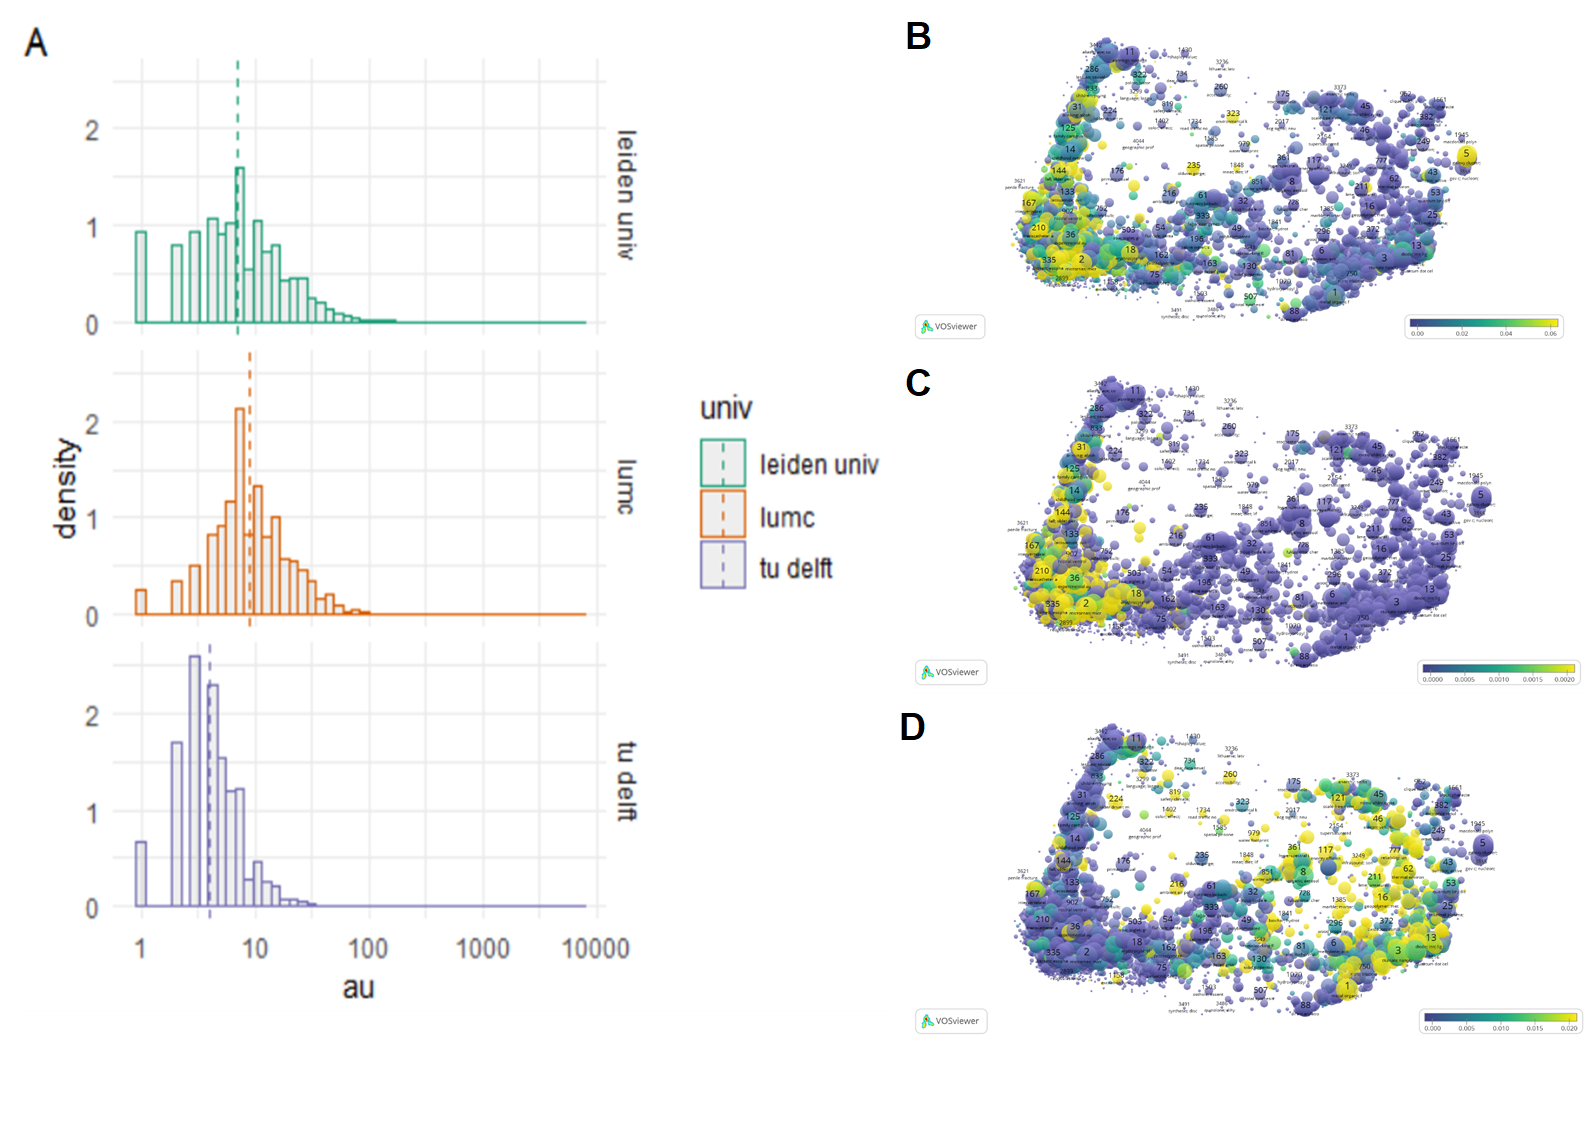
\includegraphics[width=7.14in]{C:/Users/Usuario/Documents/R/tu-case-1/figs/histogram-profiles}

\hypertarget{selection-of-case-studies}{%
\subsubsection{4.1 Selection of case
studies}\label{selection-of-case-studies}}

Six case studies will be selected. Three for each university and two by
field. The purpose of this is not only to identify differences by
discipline but also by institutional type. The fields are:

\begin{enumerate}
\def\labelenumi{\arabic{enumi}.}
\tightlist
\item
  Physics and Engineering
\item
  Social Sciences and Humanities
\item
  Biomedical Sciences
\end{enumerate}

Following I include the collaboration networks for each university and
field. I have included a threshold of at least 10 publications by
\texttt{cluster\_id}, filtered by the giant component and calculated the
betweenness centrality of each node. I have selected as seed researcher
the one with the highest centrality.

\hypertarget{physics-engineering}{%
\paragraph{Physics \& Engineering}\label{physics-engineering}}

\hypertarget{tu-delft}{%
\subparagraph{1. TU Delft}\label{tu-delft}}

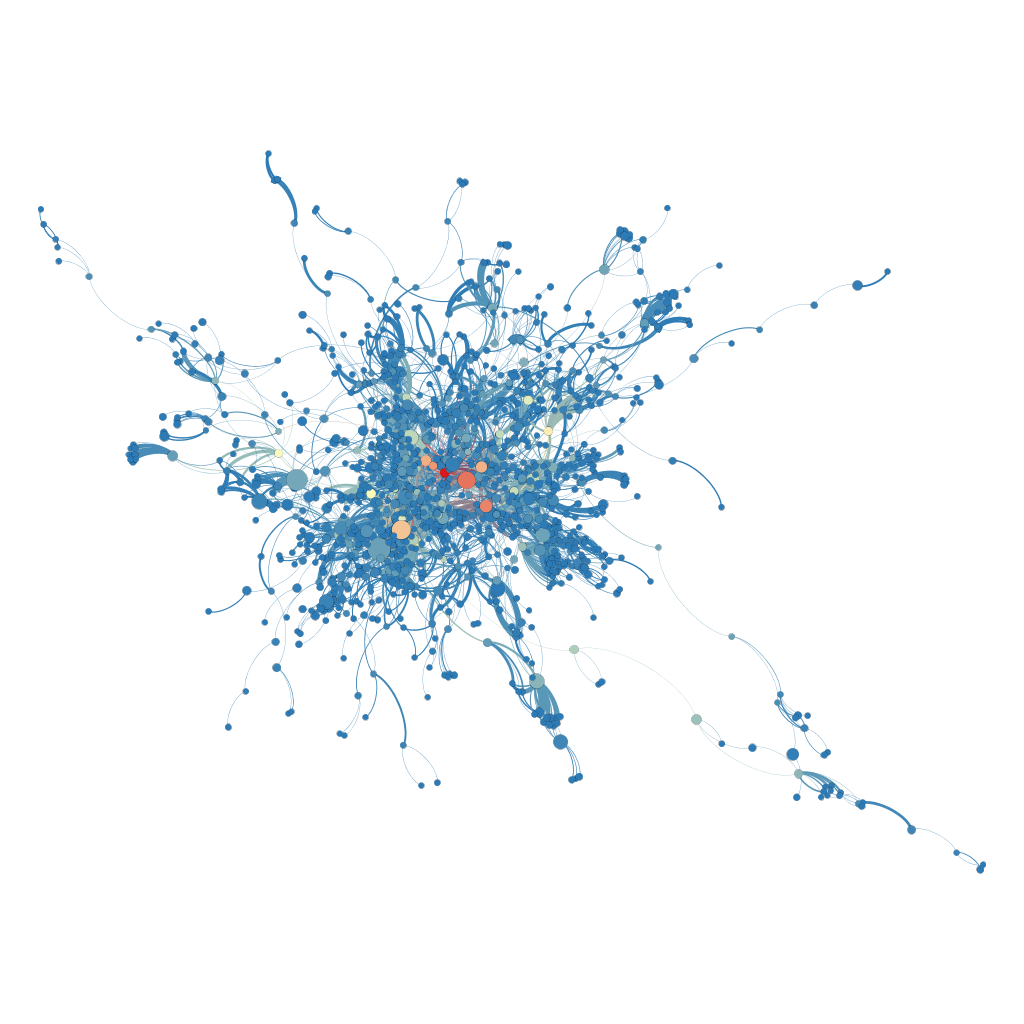
\includegraphics[width=3.41in]{C:/Users/Usuario/Documents/R/tu-case-1/figs/tu_phys_betweenness}

\emph{Notes:}

\begin{itemize}
\tightlist
\item
  1260 nodes (21.9\% visible); 4702 edges (27.1\% visible).
\item
  \texttt{cluster\_id} with highest betweenness = 33800547; Betweenness
  centrality: 0.11; Total publications = 159; Age = 32
\item
  Name: Frans D. Tichelaar; First year: 1986; Last year: 2018
\item
  PURE:
  \url{https://pure.tudelft.nl/portal/en/persons/fd-tichelaar(56299c58-b6ec-478b-b188-b8744b69d954).html}
\item
  Institution: \url{http://nchrem.nl/people/dr-ir-f-d-tichelaar-frans/}
\end{itemize}

\hypertarget{leiden-univ}{%
\subparagraph{2. Leiden Univ}\label{leiden-univ}}

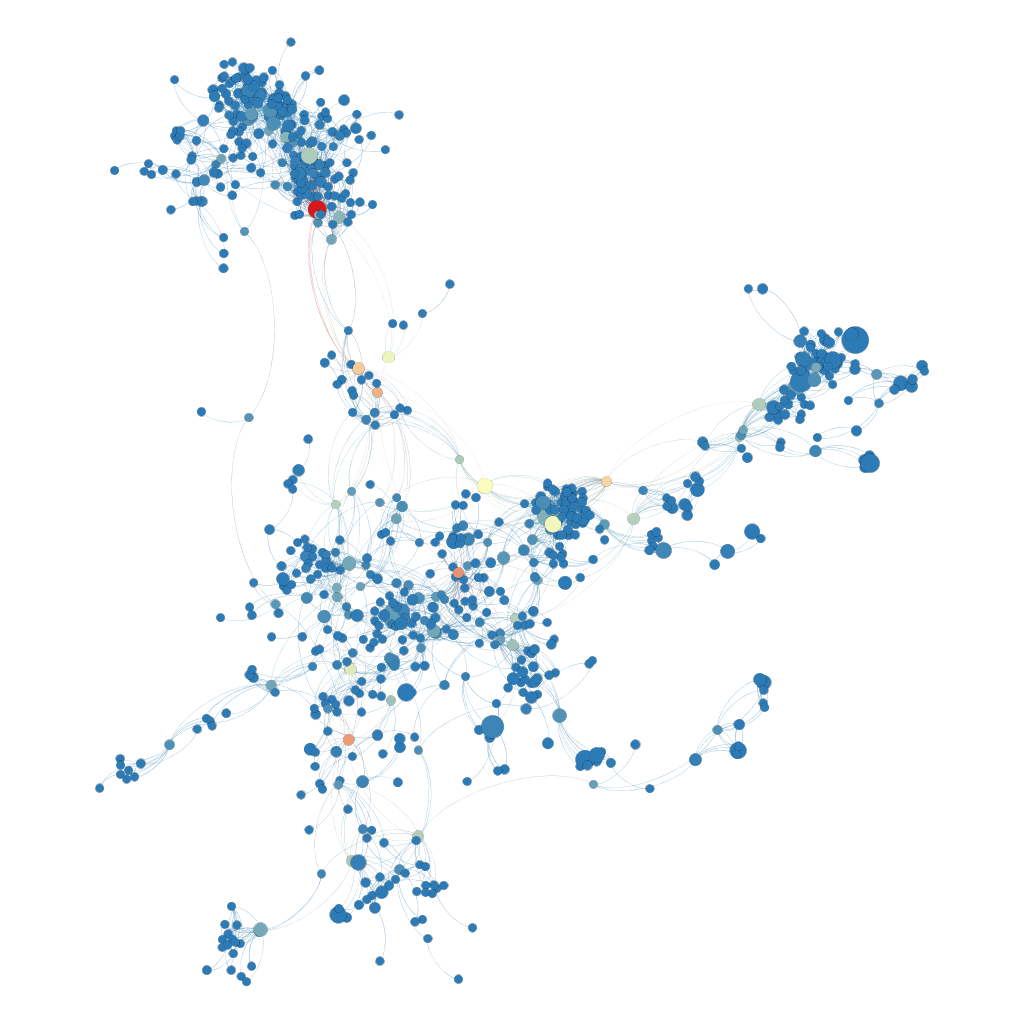
\includegraphics[width=3.41in]{C:/Users/Usuario/Documents/R/tu-case-1/figs/lu_phys_betweenness}

\emph{Notes:}

\begin{itemize}
\tightlist
\item
  765 nodes (35.1\% visible); 3409 edges (40.6\% visible).
\item
  \texttt{cluster\_id} with highest betweenness = 25501410; Betweenness
  centrality: 0.23; Total publications = 590; Age = 38
\item
  Name: Ewine F. van Dishoeck; First year: 1980; Last year: 2018
\item
  Institution:
  \url{https://local.strw.leidenuniv.nl/people/touchscreen2/persinline.php?id=16}
\item
  Personal website: \url{https://home.strw.leidenuniv.nl/~ewine/}
\end{itemize}

\hypertarget{biomedical-and-health-sciences}{%
\paragraph{Biomedical and Health
Sciences}\label{biomedical-and-health-sciences}}

\hypertarget{tu-delft-1}{%
\subparagraph{1. TU Delft}\label{tu-delft-1}}

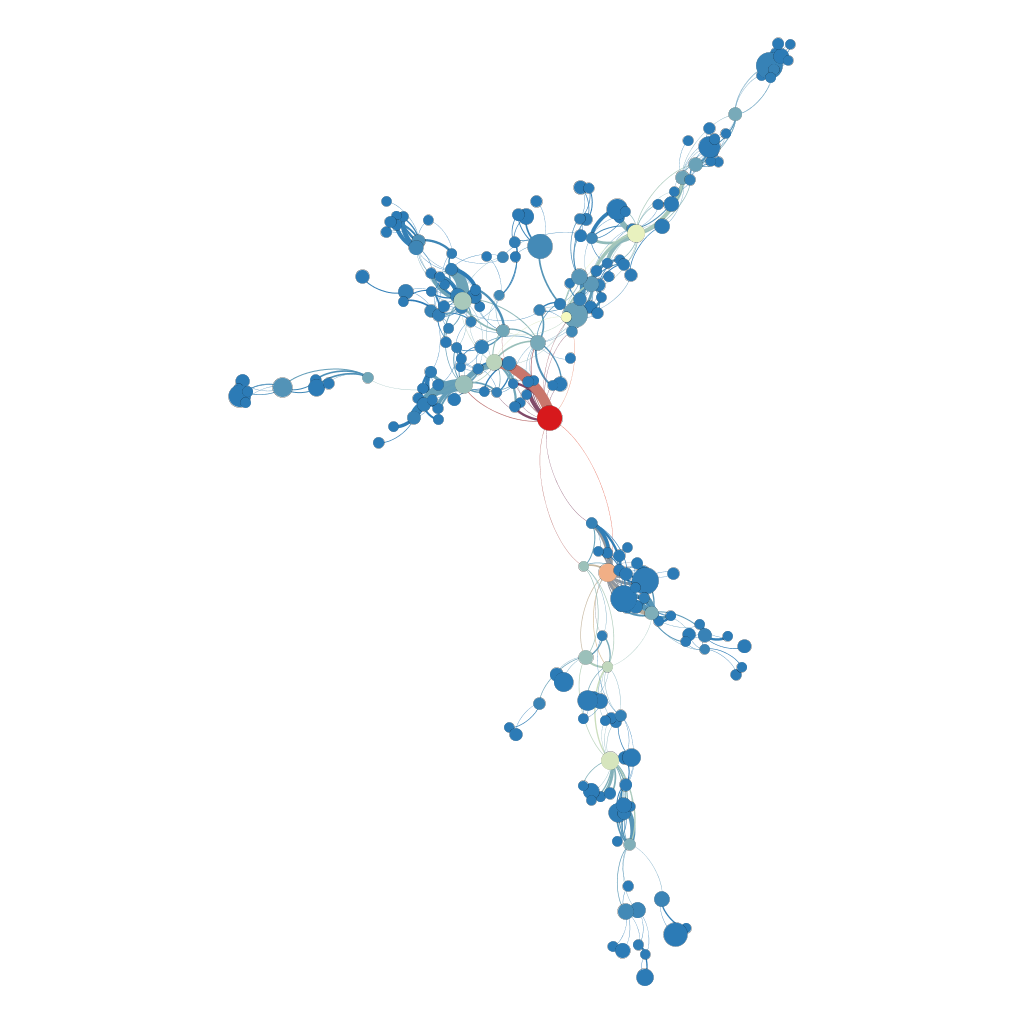
\includegraphics[width=3.41in]{C:/Users/Usuario/Documents/R/tu-case-1/figs/tu_bio_betweenness}

\emph{Notes:}

\begin{itemize}
\tightlist
\item
  214 nodes (18.9\% visible); 615 edges (25.49\% visible).
\item
  \texttt{cluster\_id} with highest betweenness = 43204348; Betweenness
  centrality: 0.50; Total publications = 341; Age = 31
\item
  Name: Harrie H. Weinans; First year: 1987; Last year: 2018
\item
  Google Profile:
  \url{https://scholar.google.com/citations?user=di4NUp8AAAAJ\&hl=en}
\item
  PURE:
  \url{https://pure.tudelft.nl/portal/en/persons/hh-weinans(f31bd75b-1863-4202-b64b-7356538284a7)/publications.html}
\item
  Co-affiliated to UMC Utrecht and TU Delft.
\end{itemize}

\hypertarget{leiden-univ-1}{%
\subparagraph{2. Leiden Univ}\label{leiden-univ-1}}

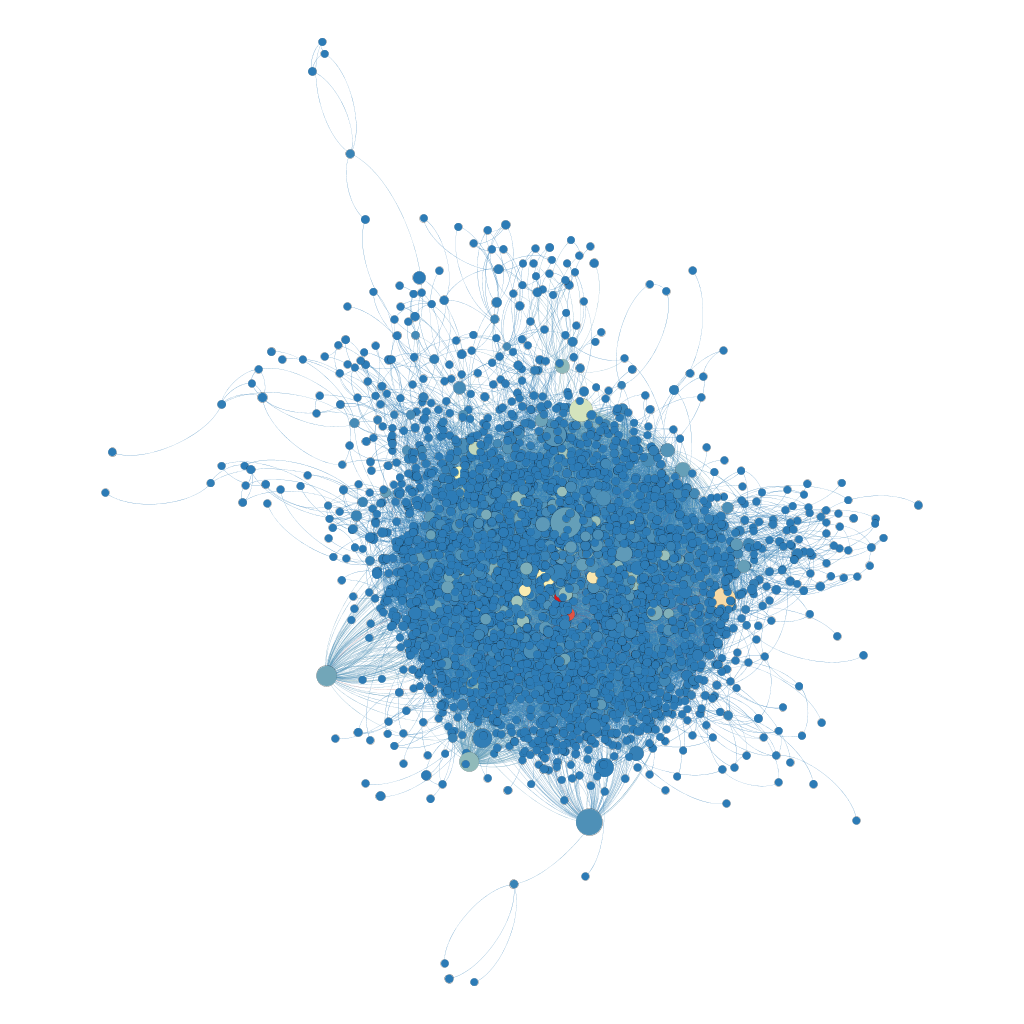
\includegraphics[width=3.41in]{C:/Users/Usuario/Documents/R/tu-case-1/figs/lu_bio_betweenness}

\emph{Notes:}

\begin{itemize}
\tightlist
\item
  Due to the density of the network the selected node can scarcely be
  seen.
\item
  3304 nodes (38.8\% visible); 43647 edges (59.6\% visible).
\item
  \texttt{cluster\_id} with highest betweenness = 19936939; Betweenness
  centrality: 0.47; Total publications = 185; Age = 27
\item
  Name: Ron Wolterbeek; First year: 1991; Last year: 2018
\item
  Institution: \url{https://www.lumc.nl/org/bds/medewerkers/rwolterbeek}
\item
  Affiliated to LUMC.
\end{itemize}

\hypertarget{social-sciences-and-humanities}{%
\paragraph{Social Sciences and
Humanities}\label{social-sciences-and-humanities}}

\hypertarget{tu-delft-2}{%
\subparagraph{1. TU Delft}\label{tu-delft-2}}

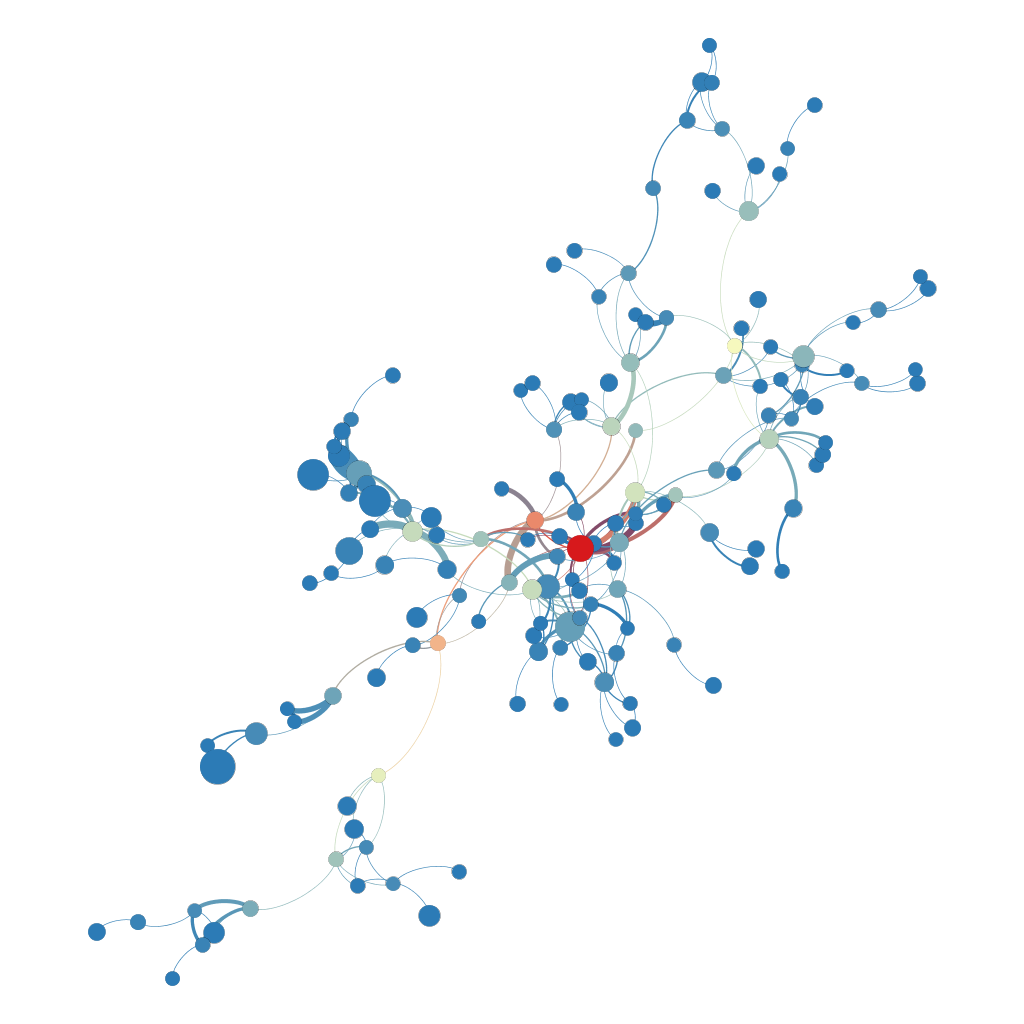
\includegraphics[width=3.41in]{C:/Users/Usuario/Documents/R/tu-case-1/figs/tu_soc_betweenness}

\emph{Notes:}

\begin{itemize}
\tightlist
\item
  151 nodes (12.6\% visible); 281 edges (15.8\% visible).
\item
  \texttt{cluster\_id} with highest betweenness = 12392841; Betweenness
  centrality: 0.41; Total publications = 134; Age = 18
\item
  Name: Bert van Wee; First year: 1999; Last year: 2018
\item
  Google Profile:
  \url{https://scholar.google.es/citations?user=dYUiqMYAAAAJ\&hl=en}
\item
  Institution:
  \url{https://www.tudelft.nl/en/tpm/about-the-faculty/departments/engineering-systems-and-services/people/full-professors/profdr-gp-bert-van-wee/}
\end{itemize}

\hypertarget{leiden-univ-2}{%
\subparagraph{2. Leiden Univ}\label{leiden-univ-2}}

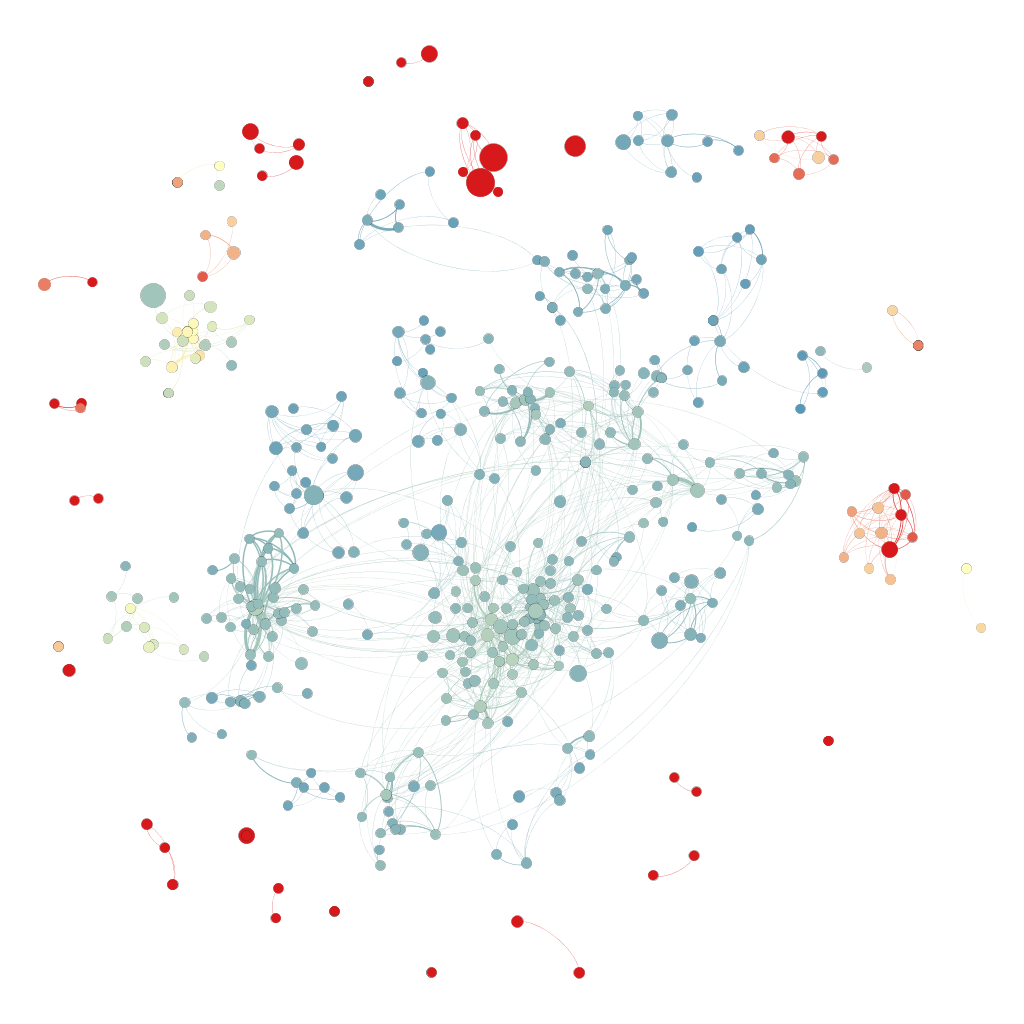
\includegraphics[width=3.41in]{C:/Users/Usuario/Documents/R/tu-case-1/figs/lu_soc_betweenness}

\emph{Notes:}

In this case, the selection of the seed researcher was not based on
network indicator. The network above has the OpenOrd layout (instead of
Yi ) and K-Core=1 group. The main issue here is that this field is
largely populated by biomedical scientists and psychologists and
psychiatrists, fields which are not good representations of Social
Sciences and Humanities. What I have done is looked at those pairs of
scholars with the highest shares of co-authored papers and go down the
list until I found someone who was not from these fields nor from CWTS
(Ludo and Nees are the third pair with more co-authored papers)

\begin{itemize}
\tightlist
\item
  478 nodes (26.5\% visible); 1294 edges (43.1\% visible).
\item
  \texttt{cluster\_id} selected = 36871407; Betweenness centrality:
  0.00; Total publications = 78; Age = 18
\item
  Name: Judi Mesman; First year: 2000; Last year: 2018
\item
  Institution:
  \url{https://www.universiteitleiden.nl/en/staffmembers/judi-mesman/publications\#tab-1}
\item
  Lab1: \url{http://www.diversityinparenting.nl/}
\item
  Lab2: \url{https://www.societalchallengeslab.com/}
\end{itemize}


\end{document}
